
\documentclass[10pt, a4paper, twoside]{article}
\usepackage[utf8]{inputenc}
\usepackage{authblk}
\usepackage{multicol}
\usepackage{abstract}
\usepackage{xcolor}
%\usepackage[a4paper, total={6in, 8in}]{geometry}
\usepackage[top=1.25in, bottom=1.25in, left=1in, right=1in]{geometry}
\usepackage{graphicx}
\usepackage{newfloat}
\usepackage{hyperref}
\usepackage{csvsimple}
\usepackage{lscape}
\usepackage{makecell}
\usepackage{fancyhdr}
\usepackage{amsmath}

\DeclareFloatingEnvironment[name={Supplementary Figure},fileext=lsf,listname={List of Supplementary Figures}]{suppfigure}

\setlength{\columnsep}{1cm}

\pagestyle{fancy}

\graphicspath{{../Figures/}}
\title{Impact of cross-border-associated cases on the SARS-CoV-2 epidemic in Switzerland from June to September 2020}
\renewcommand*{\Authfont}{\small}
\author[1]{Martina L. Reichmuth}
\author[1,2]{Emma B. Hodcroft}
\author[1,3]{Julien Riou}
\author[2,4]{Richard A. Neher}
\author[5,6]{Niel Hens}
\author[1*]{Christian L. Althaus}

\renewcommand*{\Affilfont}{\scriptsize}
\affil[1]{Institute of Social and Preventive Medicine, University of Bern, Bern, Switzerland}
\affil[2]{Swiss Institute of Bioinformatics, Basel, Switzerland}
\affil[3]{Federal Office of Public Health, Liebefeld, Switzerland}
\affil[4]{Biozentrum, University of Basel, Basel, Switzerland}
\affil[5]{Interuniversity Institute for Biostatistics and statistical Bioinformatics, Data Science Institute, Hasselt University, Hasselt, Belgium}
\affil[6]{Centre for Health Economics Research and Modelling Infectious Diseases, Vaccine and Infectious Disease Institute, University of Antwerp, Antwerp, Belgium}
\affil[*]{Correspondence: christian.althaus@ispm.unibe.ch}


\date{}
\pagenumbering{arabic}
\begin{document}
\maketitle
\normalsize
\begin{abstract}
\noindent 
\textbf{Introduction:} In Switzerland, the severe acute respiratory syndrome coronavirus 2 (SARS-CoV-2) epidemic grew from a few dozen confirmed cases to several hundred cases per day during summer 2020.
During this time, travelling to higher incidence countries might lead to more SARS-CoV-2 cases.
Holiday travel without quarantine or having tested negative for SARS-CoV-2 was largely allowed.
The impact of potential cross-border-associated cases (imports) on the national epidemic dynamics remained unclear. 
Our objective was to assess the impact of imports on the SARS-CoV-2 epidemic in Switzerland during summer 2020.\\
\textbf{Method:} We analysed individual data on confirmed SARS-CoV-2 cases reported by the Swiss Federal Office of Public Health (FOPH) from 1 June to 30 September 2020. 
We used a stochastic branching process model that accounts for super-spreading of SARS-CoV-2 to simulate epidemic trajectories in absence and presence of cross-border-associated cases.\\
\textbf{Results:} From June to September 2020, a total of 23,199 SARS-CoV-2 cases were reported in Switzerland. 
For 12,259 (53\%) of these cases, the most likely country of exposure was available and 3,304 (27\%) declared that exposure was most likely abroad. 
Assuming that all cases were infected locally (no imports), we estimated the effective reproduction number $\mathcal{R}_e$ above the critical threshold of one (1.08, 95\%-credible interval, CrI: 1.05-1.11).
In contrast, we estimated $\mathcal{R}_e$ to 0.84 (95\%-CI: 0.81-0.87) if imports were taken into account.\\
\textbf{Discussion:} In Switzerland, imports have had a considerable impact on the national dynamics and can explain the growth of the SARS-CoV-2 epidemic during summer 2020. 

\clearpage
\end{abstract}



\begin{multicols}{2}
\section{Introduction}

\rhead{Confidential, please delete!}
\lhead{ }
%Need to be more precise. Focus on problem at beginning.
At the beginning of 2020 the severe acute respiratory syndrome coronavirus 2 (SARS-CoV-2) spread to many countries around the world, which shortly afterwards led to the SARS-CoV-2 pandemic.\cite{worobey_emergence_2020}
%Since then many have been aiming to minimise the SARS-CoV-2 cases and associated deaths.
Cross-border-associated cases were most likely responsible for many new introductions that resulted in local outbreaks around the wolrd.\cite{russell_effect_2021}
With a high number of introductions, i.e., cross-border-associated cases, the local effective reproductive number $\mathcal{R}_e$ was likely overestimated.\cite{roberts_early_2011}
The $\mathcal{R}_e$ represents the average number of secondary cases per infectious case in a population with a given state of susceptibility and particular measures of prevention and control in specific place excluding new introductions.
Thus, cross-border-associated cases should not effect the (local) $\mathcal{R}_e$.
However, estimations of $\mathcal{R}_e$ do generally not exclude cross-border-associated cases.
Between June and September, 2020, the Swiss Federal Office of Public Health (SFOPH) reported a slow increase in the number of reported SARS-CoV-2 cases from a few dozen per day to several hundreds.
%This increase occurred despite the warm and dry weather in the northern hemisphere, which should have hindered the epidemic from spreading as fast.\cite{neher_potential_2020} 
The impact of cross-border-associated on the increased SARS-CoV-2 incidence in Switzerland in summer 2020 remained largely unknown.

After unprecedented measures - closure of public institutions, leisure facilities, schools and universities, mandatory home office and closing of borders -  in April and May 2020, Switzerland and other European countries reopened their borders allowing for travel.
Switzerland reopened borders on 15 June 2020 to countries of the Schengen area.\cite{federal_council_coronavirus_2020}
With 8,5 millions citizens Switzerland is a relatively small country in the heart of Europe with borders to Germany, France, Italy, Austria and Liechtenstein.
Moreover, Swiss like to travel and many different countries were easily visited by the Swiss and conversely, many citizens from other countries might visited Switzerland.
Around 80\% said that traveling is part of their holidays.\cite{heim_dreivon_2020}
Before the SARS-CoV-2 pandemic, around 49\% planned to travel abroad, this reduced to 15\% in June 2020.\cite{bosshardt_schweiz_2020}
For many Swiss, the SARS-CoV-2 incidence of holiday destinations was crucial for their decision.\cite{bosshardt_schweiz_2020}
A survey study showed that around 4\% were planning to go to Germany, 3\% to France and 2\% to Italy or Austria.\cite{bosshardt_schweiz_2020}
More distant holiday destinations like Spain or Greece was planned to visit by less than 1\%.\cite{bosshardt_schweiz_2020}

In the absence of travel restrictions, cross-border-associated cases are to be expected.\cite{russell_effect_2021} 
A phylogenetic analysis assessed the occurrence of cross-border-associated cases.\cite{hodcroft_emergence_2020}
In summer 2020, the SARS-CoV-2 variant, 20E (EU1), that most likely originated in Spain spread multiple times to several other countries including Switzerland.\cite{hodcroft_emergence_2020}
It revealed failures in travel control during the pandemic, e.g. there were travels to higher incidence countries without adequate contact tracing and containment.\cite{hodcroft_emergence_2020}
Introductions to many countries around the world were also seen for B.1.1.7, B.1.1.28.1, B.1.351, and B.1.617.\cite{davies_estimated_2021,faria_genomics_2021,tegally_detection_2021,cherian_convergent_2021} 
Highlighting the need of global collaboration in combating the pandemic and importance of large genomic surveillance.
First to stop the introduction of variants of concern (VOC) and second to control the spread of VOCs.

Previously, stochastic branching process models were used to find trajectories that were consistent with surveillance data.\cite{althaus_ebola_2015,riou_pattern_2020}
It helped to determine epidemiological parameters such as the $\mathcal{R}_e$ or the over-dispersion parameter.\cite{althaus_ebola_2015,riou_pattern_2020}
In this study, we used a stochastic branching process model to find the most plausible trajectories of the summer 2020 epidemic in Switzerland.
We analysed confirmed SARS-CoV-2 cases and the reported most likely country of their exposure, i.e., where cases had been the last 14 days before they got tested or began to have symptoms.
Then we selected epidemic trajectories that were consistent with data reported by the SFOPH.
We quantified the impact of cross-border-associated cases on $\mathcal{R}_e$ in Switzerland between June and September 2020.

\section{Method}

\subsection{Data}
For the purpose of this study, we analysed surveillance data of the SARS-CoV-2 epidemic in Switzerland from 1 June to 30 September 2020. 
We used individual data on positive cases reported by the SFOPH. 
Data included for each case: age, sex, date of diagnosis or registration, and the most likely country of exposure, i.e., a country where they had been within the last 14 days before they got tested or began to have symptoms.
We considered the 23 most frequently reported countries of exposure including Switzerland (Tabe \ref{t2}).
Other countries (mentioned less than ten times) were grouped to 'others'.
We preformed a linear regression to estimate the differences in age (in 1 years steps) between individuals that had been exposed in different countries.
Further, we grouped individuals into three categories based on their age: $<$21 years, 21-64 years and  $>$64 years.
\textit{'Our World in Data'} was used to present incidence for all 23 countries (variable: \textit{'new\_cases\_smoothed\_per\_million'}; Supplementary Figure \ref{sf1}).\cite{hasell_cross-country_2020}
Additionally, we calculated the incidence for Switzerland.%maybe delete these 3 sentences?
Therefore, we calculated incidence of confirmed cases for each day including one week, i.e. mean of three days before and after the date of interest.
The estimated mean of incidence was divided by 8,697,905 (number of Swiss citizens see \href{https://www.worldometers.info/world-population/switzerland-population/}{here}) and multiplied by 100,000.


\subsection{Inferring growth rates and $\mathcal{R}_e$}\label{marker}
We fitted a negative binomial generalised linear model to the daily number of confirmed cases of SARS-CoV-2 infections $y$ starting on 1 June to 30 September 2020:
\begin{equation}
	\log(\text E(y|t)) = a + r t,
\end{equation}
where $a$ was an intercept, $r$ is a growth rate and $t$ was the time in days.
Thus, we estimated a constant growth rate $r$ for the whole study period.
Growth rate and reproductive number can be derived from each other taking into account the generation time, i.e. time between the infection of a primary case and one of its secondary cases.\cite{wallinga_how_2007,krauer_heterogeneity_2016,svensson_note_2007}
This approach assumes that acquired immunity was minimal during the period of interest, and that  the reporting rate was stable.
%Until 31 May 2020, 30,883 SARS-CoV-2 cases were reported by the SFOPH.\cite{federal_office_of_public_health_coronavirus_nodate}
We assumed a gamma distributed generation time with shape $\alpha$ and rate $\beta$, leading to the relation:
\begin{equation}
	\mathcal{R}_e = (1 + \frac{r}{\beta} )^\alpha.
\end{equation}
For SARS-CoV-2, a mean generation time of $\mu= 5.2$ days with a standard deviation of $\sigma = 1.72$ was reported.\cite{ganyani_estimating_2020}
Parameters $\alpha$ (gamma shape) and $\beta$ (gamma rate) were given by $\mu$ and $\sigma$ as $\frac{\mu^2}{\sigma^2 }$ and $\frac{\mu}{\sigma^2}$, respectively.

\subsection{Epidemic simulations}
We simulated epidemics for 1 June to 30 September 2020 using a stochastic branching process model that accounted for super-spreading in transmission of SARS-CoV-2.\cite{riou_pattern_2020}
The branching process was based on a negative-binomial distribution for the distribution of secondary cases, with a mean of $\mathcal{R}_e$ and over-dispersion parameter $k$.
The generation time for each transmission event was sampled from a gamma distribution as described in the previous section.

Within our branching process model we considered different values for $\mathcal{R}_e$, for $k$ and for the seed -- the number of infectious individuals during the week preceding the start of the simulation (Table \ref{t1}).
We considered a prior distribution for $\mathcal{R}_e$ from 0.5 to 1.5.
For $k$, we considered values between 0.49 and 0.52 as estimated from contact tracing data in India\cite{laxminarayan_epidemiology_2020}, and in sensitivity analyses we also considered values of 0.1 and 1.\cite{taube_open-access_2021}
For the seed, we used the estimate of the $E(y|t))$ for $t_{-7}$ to $t_{-1}$ in equation (1) with its 95\%-predictive interval, resulting in values from 12 to 33 cases per day.
For each trajectory seeds for $t_{-7}$ to $t_{-1}$  were randomly selected from a uniform distribution ranging from 12 to 33 cases per day.
This resulted in a total of 94 to 222 cases from 25 to 31 May 2020, where the SFOPH reported 126 cases in Switzerland this week.

The simulations proceeded as follows.
Firstly, we simulated $10^5$ epidemic trajectories with the branching process model, randomly sampling parameter values in each iteration, except for the number of cross-border-associated cases that was fixed to 0.
These trajectories only accounted for local transmission and was referred as the baseline scenario.
We removed trajectories leading to a cumulative incidence over 10$^6$ (43 times more than the confirmed cumulative incidence).

Secondly, we accounted for cross-border-associated cases and added these to the baseline scenario.
In these scenarios, cross-border-associated cases were added to each trajectory according to the date of test (Figure \ref{f1}d).
Cross-border-associated cases were equally likely to transmit, i.e., initiating new branches of local transmission, as all other cases.

The SFOPH reported 3,304 cross-border-associated cases during the study period, but the information on the country of exposure was missing for 10,940 cases.
For 12,259 out of 23,199 (53\%, the extrapolation factor) information was available.
To capture the uncertainty of missing information we considered three different scenarios that account for cross-border-associated cases.
The most plausible scenario a) considered missing of the country of exposure and the corresponding lack of the exact number of cross-border-associated cases as random by using following calculation: reported cross-border-associated cases per day * extrapolation factor.
In the lower limit scenario b) cross-border cases were less likely among the missing exposure countries by using following calculation: reported cross-border-associated cases per day * extrapolation factor * 2/3.
Contrary, in the upper limit scenario c) cross-border cases were more likely among the missing exposure countries by using following calculation: reported cross-border-associated cases per day * extrapolation factor * 3/2.

\end{multicols}
\begin{table}
\centering
\begingroup\footnotesize
\begin{tabular}{clll}
	\hline
	Parameter & Description & Values considered & Sampling strategy\\
	\hline
	$\mathcal{R}_e$ & Effective reproductive number & 0.5 - 1.5 & $10^5$ uniformly distributed\\
	$k$ & Over-dispersion parameter & 0.49 - 0.52 & $10^5$ normally distributed\\
	$n$ & Seeds & 12 - 32 per day & uniformly distributed\\
	$I$ & Imports & baseline; a); b); c) & four scenarios\\
	\hline
\end{tabular}
\endgroup
\caption{Prior distributions of the parameters used to simulate the epidemic trajectories.} 
\label{t1}
\end{table}
\begin{multicols}{2}

\subsection{Inference}
Following the principles of approximate Bayesian computation (ABC), simulated epidemic trajectories were rejected when the cumulative incidence and final incidence fell outside of predefined ranges.
Predefined ranges for cumulative incidence and final incidence were constructed using SFOPH reports on confirmed cases.
We used ($10^4$ simulations of) random negative binomial model to obtain 95\%-credible interval (CI) of (I) the cumulative incidence from 1 June to 30 September 2020, and (II) the final incidence from 24 to 30 September 2020 divided by 7.
The random negative binomial model was calibrated with the standard error of equation (1) and (I) the cumulative incidence for the period of interest or (II) the cumulative incidence for the last seven days, repsectively.

All analyses were preformed using $R~v.4.0$ with following packages \texttt{MASS, MCMCglmm, doParallel, foreach, lubridate, reshape2, ggplot2, ggpubr, grid, gridExtra, RColorBrewer}.\cite{r_core_team_r_2020}%venables_modern_2002

\section{Results}
In total 23,199 cases were confirmed by the SFOPH between 1 June to 30 September 2020 (Table \ref{t2}). 
Of them, 13,929 (48\%) were female and 14,985 (52\%) were male.
For nine individuals the gender was not known.
For 12,259 (53\%) cases the most likely country of exposure was reported.
Of them, 3,304 (27\%) reported an exposure abroad (Table \ref{t2}); Figure \ref{f1}).
The peak of reported cross-border-associated was on 6 September 2020 with 105 cases (Figure \ref{f1}c,d).
Of all exposures that were likely to have happened abroad 1,562 (44\%) were female and 2,000 (56\%) were male.

\end{multicols}
%\begin{landscape}
%\global\pdfpageattr\expandafter{\the\pdfpageattr/Rotate 90}
%\input{{../data/table2.tex}}
%\end{landscape}
%\begin{multicols}{2}
%\global\pdfpageattr\expandafter{\the\pdfpageattr/Rotate 0}
\begin{table}
\begingroup\footnotesize
\begin{tabular}{llrllll}
  \hline
Country &\makecell{Incidence\\per $10^6$\\median (range)} &\makecell{Confirmed\\cases} &\makecell{Known\\exposure\\(in \%)} &\makecell{Cases\\abroad\\(in \%)} &\makecell{Age in years\\median (IQR)} &\makecell{Mandatory\\quarantine} \\ 
  \hline
All reported cases &  -  & 23199 &  -  &  -  & 34 (24-50) &  -  \\ 
  Cross-border-associated &  -  & 3304 & 26.95 & 100.00 & 31 (23-48) &  -  \\ 
  Switzerland & 17.1 (1.7 - 50.9) & 8955 & 73.05 &  -  & 35 (24-51) &  -  \\ 
  France & 15.4 (4.8 - 181.3) & 650 & 5.30 & 19.67 & 29 (23-41) & 2020-09-14 - ** \\ 
  Croatia & 19.6 (0.0 - 68.2) & 419 & 3.42 & 12.68 & 24 (21-28) & 2020-09-07 - ** \\ 
  Kosovo & 59.9 (3.3 - 122.8) & 309 & 2.52 & 9.35 & 49 (31-61) & 2020-07-06 - ** \\ 
  Italy & 5.0 (2.9 - 29.1) & 301 & 2.46 & 9.11 & 32 (24-46) & 2020-09-28 - ** \\ 
  Germany & 8.0 (2.7 - 23.7) & 184 & 1.50 & 5.57 & 37 (26-51) &  -  \\ 
  Turkey & 14.8 (10.4 - 19.9) & 169 & 1.38 & 5.12 & 39 (26-53) &  -  \\ 
  Serbia & 19.1 (4.8 - 63.6) & 153 & 1.25 & 4.63 & 46 (28-60) & 2020-07-06 - ** \\ 
  Spain & 49.2 (5.4 - 242.0) & 136 & 1.11 & 4.12 & 30 (23-42) & 2020-08-08 - ** \\ 
  Malta & 44.0 (0.0 - 137.5) & 125 & 1.02 & 3.78 & 20 (19-24) & 2020-08-20 - ** \\ 
  Greece & 5.2 (0.5 - 31.6) & 116 & 0.95 & 3.51 & 29 (25-37) &  -  \\ 
  Portugal & 31.7 (16.7 - 71.1) & 116 & 0.95 & 3.51 & 36 (25-49) & 2020-09-28 - ** \\ 
  Austria & 12.8 (2.6 - 81.2) &  65 & 0.53 & 1.97 & 35 (28-50) & 2020-09-14 - ** \\ 
  North Macedonia & 62.6 (21.7 - 77.2) &  59 & 0.48 & 1.79 & 61 (50-65) & 2020-07-06 - ** \\ 
  Albania & 36.9 (5.4 - 55.5) &  57 & 0.46 & 1.73 & 38 (27-48) & 2020-08-20 - ** \\ 
  Bosnia and Herzegovina & 73.9 (4.2 - 110.1) &  56 & 0.46 & 1.69 & 46 (30-60) & 2020-07-23 - ** \\ 
  Hungary & 1.8 (0.3 - 91.0) &  38 & 0.31 & 1.15 & 28 (23-34) & 2020-09-28 - ** \\ 
  Netherlands & 15.8 (3.0 - 172.4) &  34 & 0.28 & 1.03 & 30 (23-46) & 2020-09-28 - ** \\ 
  Poland & 12.4 (6.8 - 37.1) &  24 & 0.20 & 0.73 & 32 (31-44) &  -  \\ 
  Czech Republic & 19.8 (4.0 - 204.2) &  22 & 0.18 & 0.67 & 24 (20-33) & 2020-09-14 - ** \\ 
  Romania & 59.8 (8.0 - 82.9) &  13 & 0.11 & 0.39 & 40 (26-52) & 2020-07-23 - ** \\ 
  Slovenia & 8.7 (0.3 - 68.4) &  11 & 0.09 & 0.33 & 30 (18-34) & 2020-09-28 - ** \\ 
  UK & 14.9 (5.2 - 91.8) &  11 & 0.09 & 0.33 & 30 (20-43) & 2020-09-28 - ** \\ 
  Others &  -  & 157 & 1.28 & 4.75 & 37 (25-53) &  -  \\ 
  Abroad but unknown &  -  &  79 & 0.64 & 2.39 & 33 (26-49) &  -  \\ 
  Unknown &  -  & 10940 &  -  &  -  & 35 (25-51) &  -  \\ 
   \hline
\end{tabular}
\endgroup
\caption{Confirmed SARS-CoV-2 cases during summer 2020 regarding age and most likely country of exposure.**Mandatory quarantine did not end on 30 September 2020. Abbreviation: IQR, interquartile range} 
\label{t2}
\end{table}
\begin{multicols}{2}

The study population was 34 (interquartile range (IQR): 24-50) years and individuals that had an exposure abroad were 31 (IQR: 23-48) years (Table \ref{t2}).
Individuals who reported that Switzerland was the only country they had visited within the last 14 days were 35 (IQR: 24-51) years.
Different age categories were more likely to visit some countries during summer (Table \ref{t2}; Supplementary Figure \ref{sf2}).
Individuals were significantly younger ($<.05$) if they were exposed to SARS-CoV-2 in France, Croatia, Turkey, Serbia, Greece, Portugal, Albania, Hungary, Poland, Czech Republic, Romania, Slovenia, or the UK compared to individuals that were only in Switzerland.%Any idea how I could write this better?
Contrary, individuals were significantly older ($<.05$) if they were exposed to SARS-CoV-2 in Kosovo, Italy, Germany, Spain, Malta, Austria, North Macedonia, Bosnia and Herzegovina, Netherlands, or in other countries, abroad but unknown, or generally unknown compared to individuals that were only in Switzerland.
Tendency of crossing borders was similar regarding residency of Swiss cases (Supplementary Figure \ref{sf3}).

The incidence of 22 countries - where Swiss cases were exposed to SARS-CoV-2 - was for 81 (95\%-CI 7-122) out of 122 days higher as in Switzerland (Table \ref{t2}; Supplementary Figure \ref{sf1}).
At the beginning of June 2020, none of the 22 countries with at least a dozen returnees with a SARS-CoV-2 infection between June and September was on the list where returnees had to do quarantine.
In July 2020 the list was including five countries of 22 countries.
In August and September 3 respectively 10 additional countries were added to the list.
End of September 5 of 22 countries had not been on the list during summer.
During this time testing was not mandatory for individuals that crossed borders.


\begin{figure*}
\centering
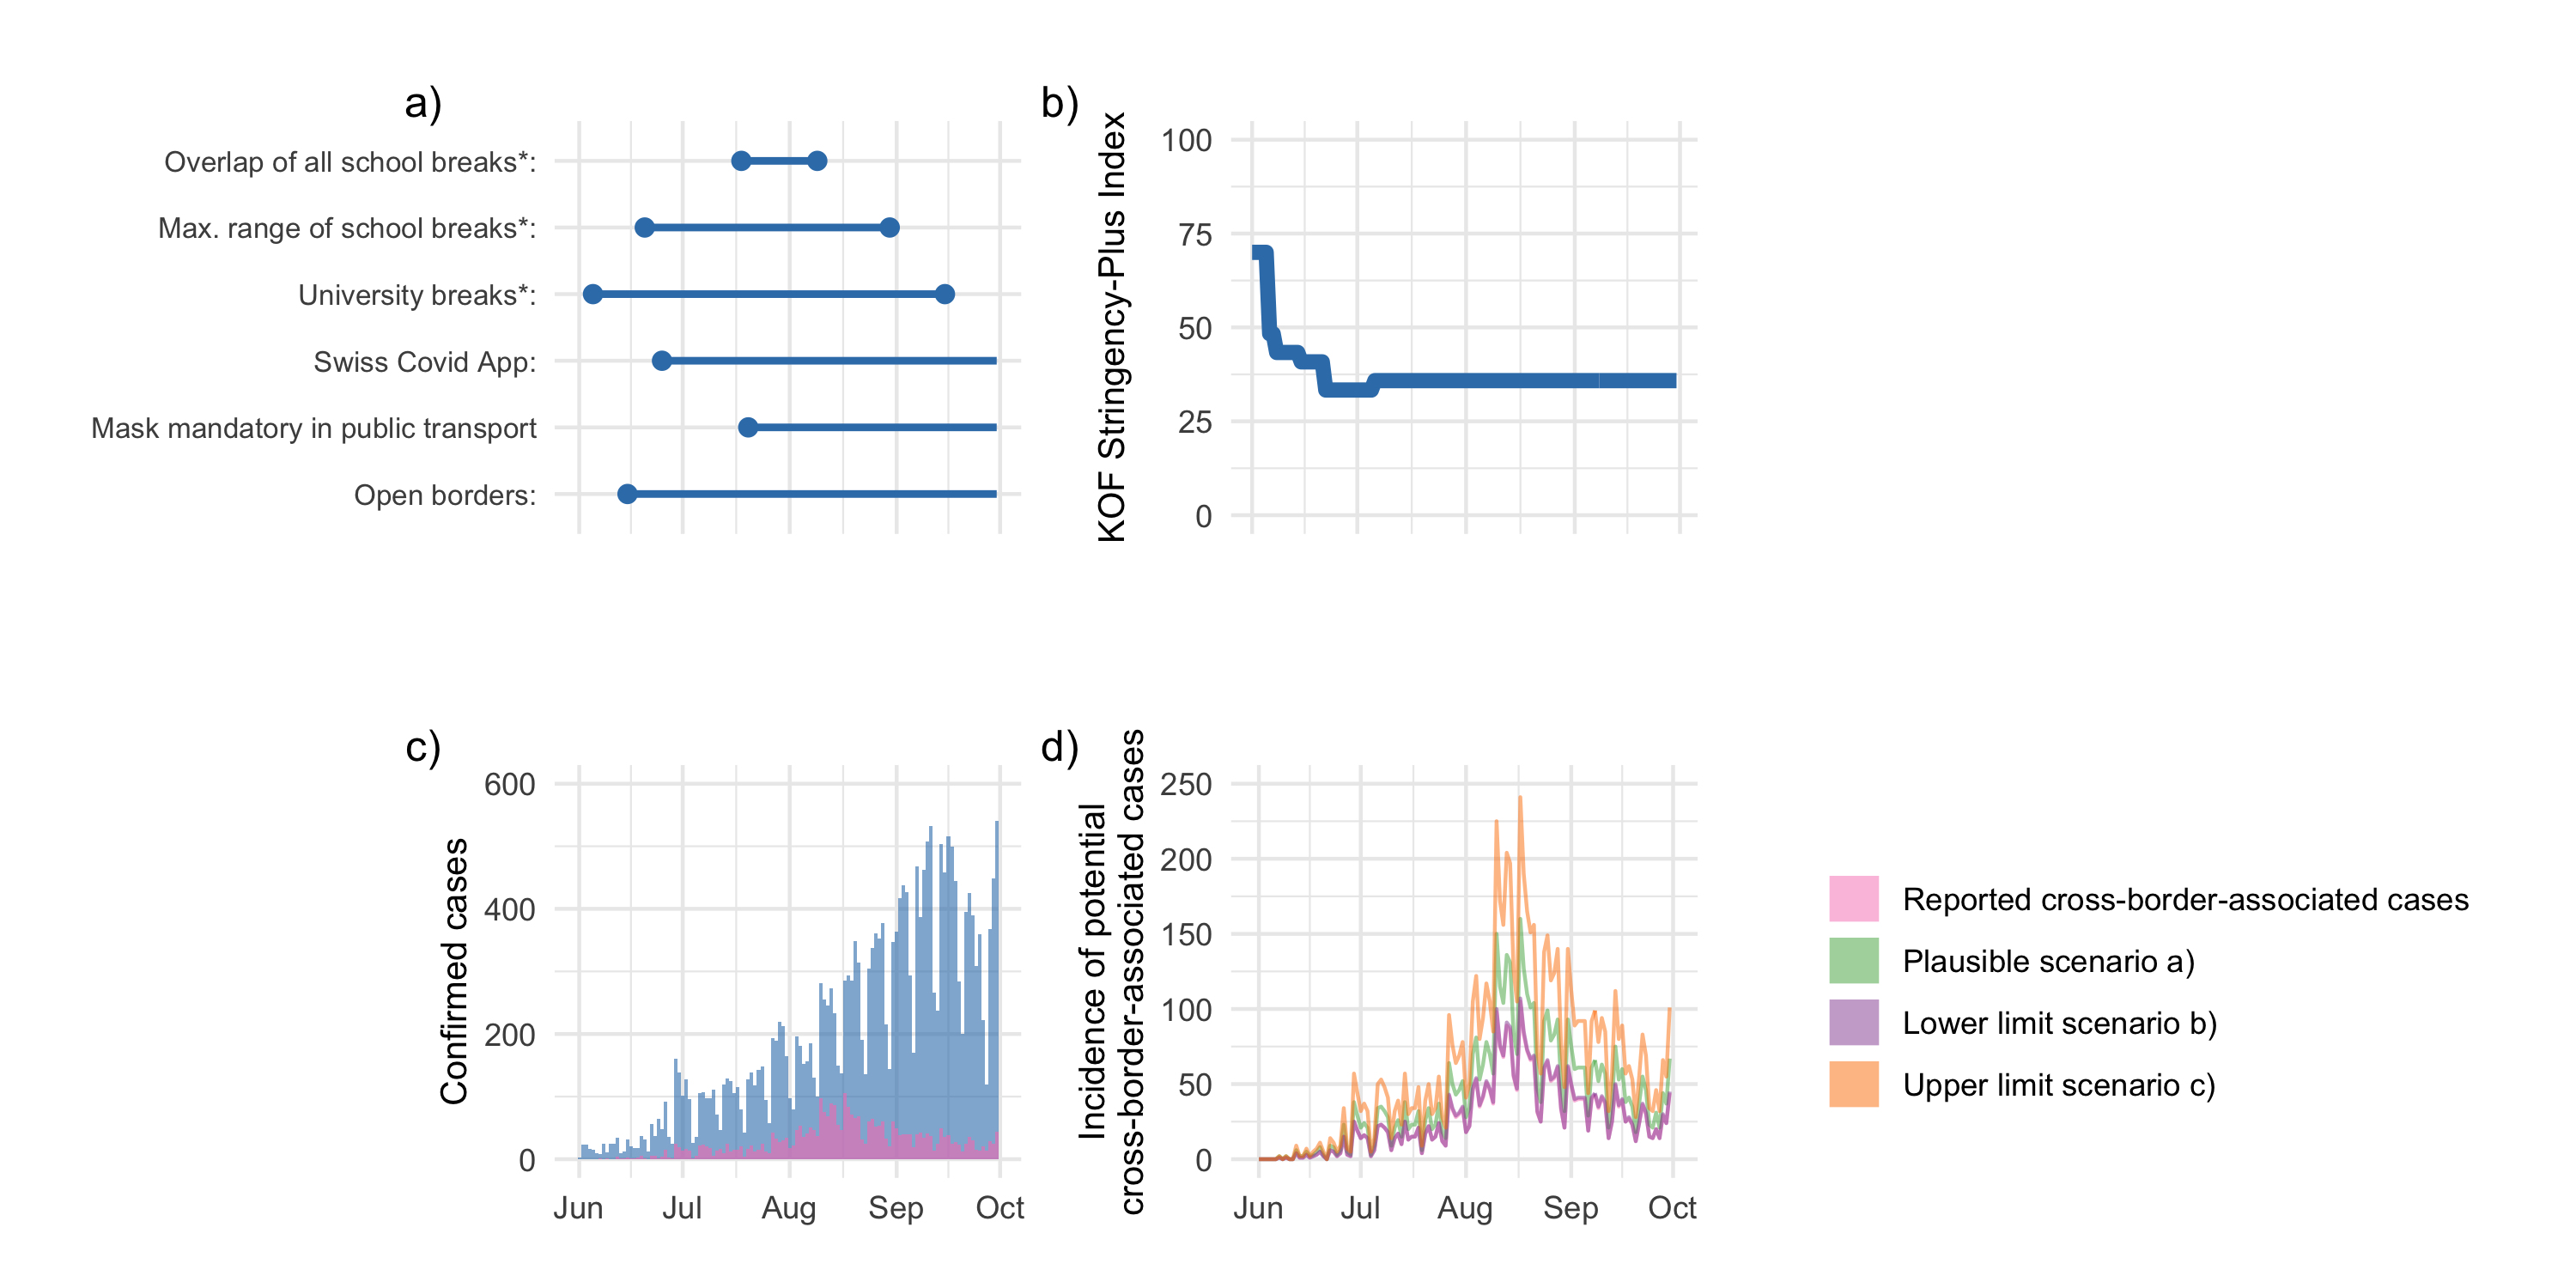
\includegraphics[scale=0.15]{Figure1_2021-06-02.png}
\caption{The Swiss SARS-CoV-2 epidemic in summer 2020.
a) Five major events that might influenced the Swiss epidemic from 1 June to 30 September 2020.
b) The \href{https://kof.ethz.ch/en/forecasts-and-indicators/indicators/kof-stringency-index.html}{KOF stringency plus index} records the stringency of COVID-19 policy measures in Switzerland over time.
The values range from 0 (= no measures) to 100 (= full lockdown).
c) Daily incidence (blue) and reported cross-border-associated cases (pink).
d) Three cross-border-associated scenarios a, b, and c that were processed with a branching process model.
*Official breaks of universities and schools might vary for different subjects and between different schools and cantons, respectively.
More details on quarantine measures in Table \ref{t2} and \href{https://www.fedlex.admin.ch/eli/cc/2021/61/de}{here}.
Abbreviations: COVID-19, coronavirus d}
\label{f1}
\end{figure*}

Beginning of June 2020 Switzerland had an incidence of 0.17 per 100,000 citizens (3 cases) and at the end of September 5.36 (540 cases; Figure \ref{f2}c).
The latter was also the maximum value during the time of interest.
Accordingly, there was an increase of cases during the summer months.
We estimated the 95\%-CI of cumulative incidence of 17,019 to 30,533 cases for the period from 1 June to 30 September 2020 (23,199 cases were reported by the SFOPH; Figure \ref{f1}a).
For the final incidence the 95\%-CI laid within 93 to 762 cases for the last day.
For a day in the last week the mean of the reported cases was 338 cases per day.

Assuming a constant growth, we estimated an epidemic growth rate of 0.03 (95\%-CI 0.02-0.03) per day and a $\mathcal{R}_e$ of 1.15 (95\%-confidence interval: 1.14-1.16) for June to September 2020.


\begin{figure*}
\centering
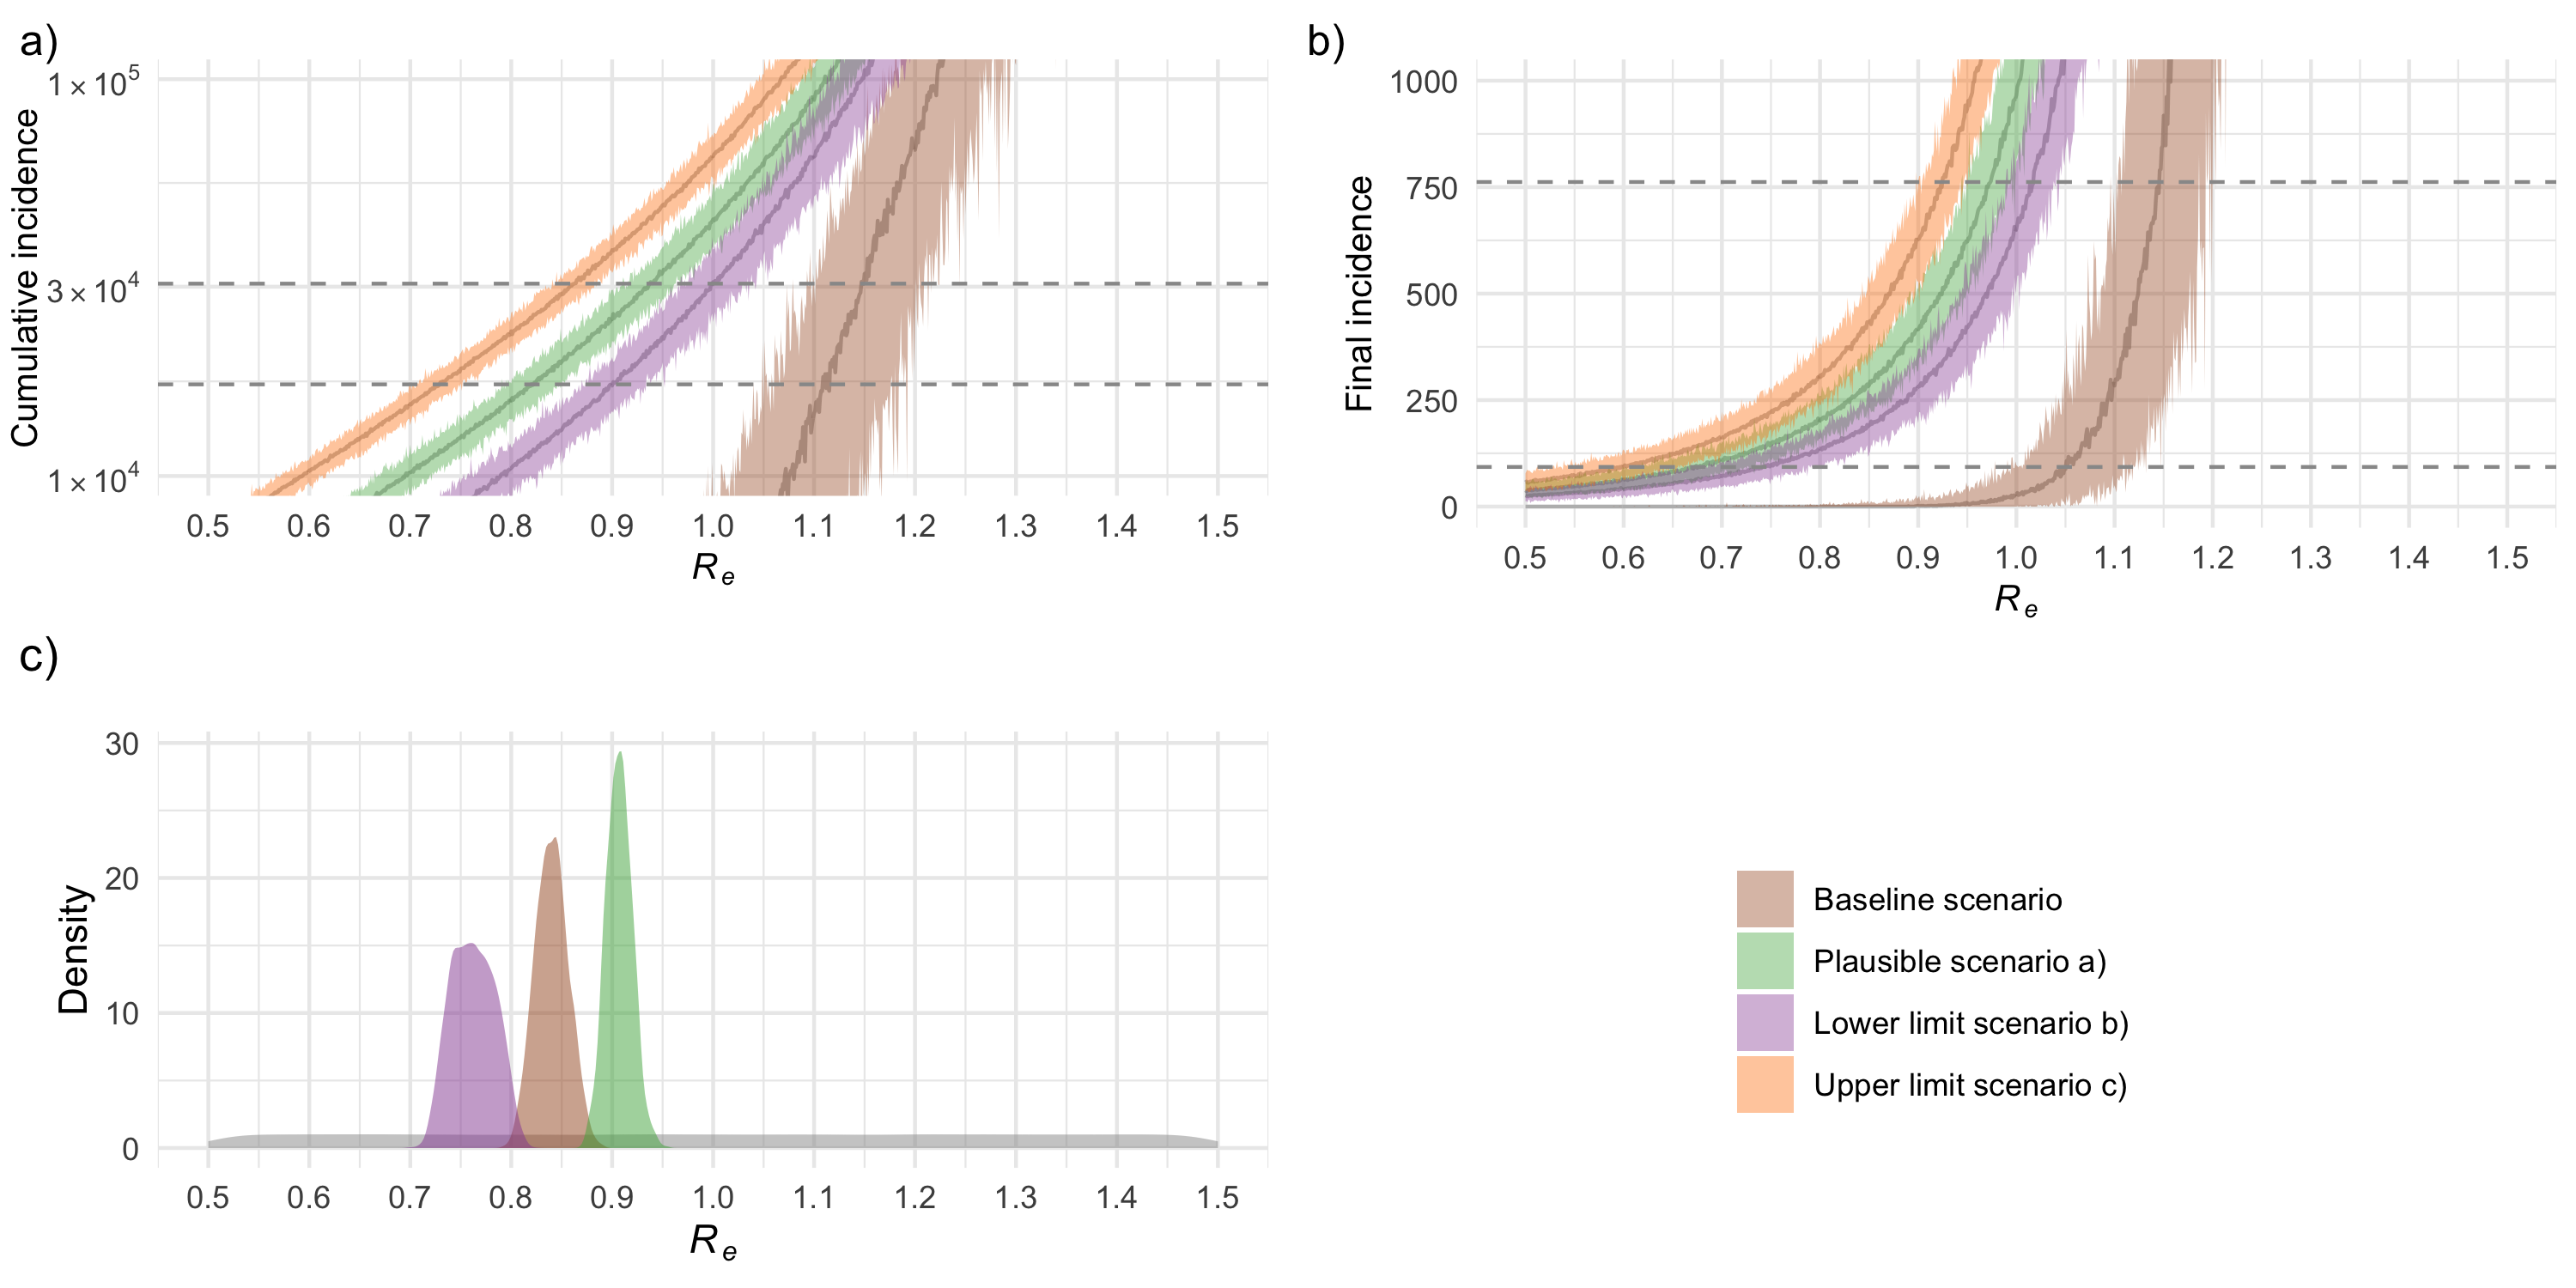
\includegraphics[scale=0.15]{Figure2_2021-06-02.png}
\caption{Impact of cross-border-associated cases on the local epidemic.
a) Curves represent credible range and median of the cumulative incidence for the baseline scenario and three scenarios that accounted for cross-border-associated cases.
Dashed lines represent 95\%-CI for the cumulative incidence during 1 June to 30 September 2020.
b) Curves represent credible range and median of the final incidence for the baseline and three models that accounted for cross-border-associated cases.
Dashed lines represent 95\%-CI of the incidence on 30 September 2020.
c) Prior and posterior distribution of $\mathcal{R}_e$ for the baseline scenario and three scenarios that accounted for cross-border-associated cases.
Abbreviations: $R_e$, the effective reproductive number; CI, credible interval}

\label{f2}
\end{figure*}

With the baseline scenario and three additional scenarios that accounted for cross-border-associated cases we simulated the Swiss epidemic.
Overall, 11,515 of $4*10^5$ (2.88\%) trajectories were within the 95\%-CI of the expected cumulative incidence and final incidence.
The baseline scenario assumed no new introductions which was not the case for the Swiss epidemic and thus, $\mathcal{R}_e$ was over-estimated.
Accounting for new introductions required to re-evaluate the intensity of local transmission, i.e. the value of $\mathcal{R}_e$, to match the observed dynamics of SARS-CoV-2 in summer 2020.
Assuming no introductions, 40 (0.04\%) trajectories were within the 95\%-CI of the expected cumulative incidence and final incidence (Figure \ref{f3}b).
The $\mathcal{R}_e$ was 1.08 (95\%-CI: 1.05-1.11; which was lower than the $\mathcal{R}_e$ derived from the equation (2) (Figure \ref{f2}c).
The baseline scenario was then extended with three scenarios a), b), and c) that included new introductions of cross-border-associated cases.
In extended models, all cases, i.e., cross-border-associated cases and local cases, were equally likely to transmit SARS-CoV-2.

Scenario a) accounted in total for 5,050 cross-border-associated cases resulting from an extrapolation of 3,304 cross-border-associated cases.
Overall, 3,690 (3.69\%) trajectories were accepted as they were within the 95\%-CI of the cumulative incidence and final incidence (Table \ref{t2}; Figure \ref{f2}; Figure \ref{f3}).
These 3,690 trajectories represented a $\mathcal{R}_e$ of 0.84 (95\%-CI: 0.81-0.87) (Figure \ref{f2}; Figure \ref{f3}).
For scenario b) and c) the number of introductions were extrapolated from the reported cross-border-associated cases and a multiplication with 2/3 and 3/2.
In total, 1,241 (1.24\%) and 6,543 (6.54\%) trajectories were within the 95\%-CI of the expected cumulative incidence and final incidence (Table \ref{t2}; Figure \ref{f2}).
These 1,241 and 6,543 trajectories represented a $\mathcal{R}_e$ of 0.91 (95\%-CI: 0.88-0.93) and $\mathcal{R}_e$ of 0.76 (95\%-CI: 0.72-0.80) (Figure \ref{f2}; Figure \ref{f3}).

Our results did not depend on the dispersion parameter $k$.
Same $\mathcal{R}_e$ values were estimated for all four scenarios if we set $k = 0.1$ and $k = 1$.

\begin{figure*}
\centering
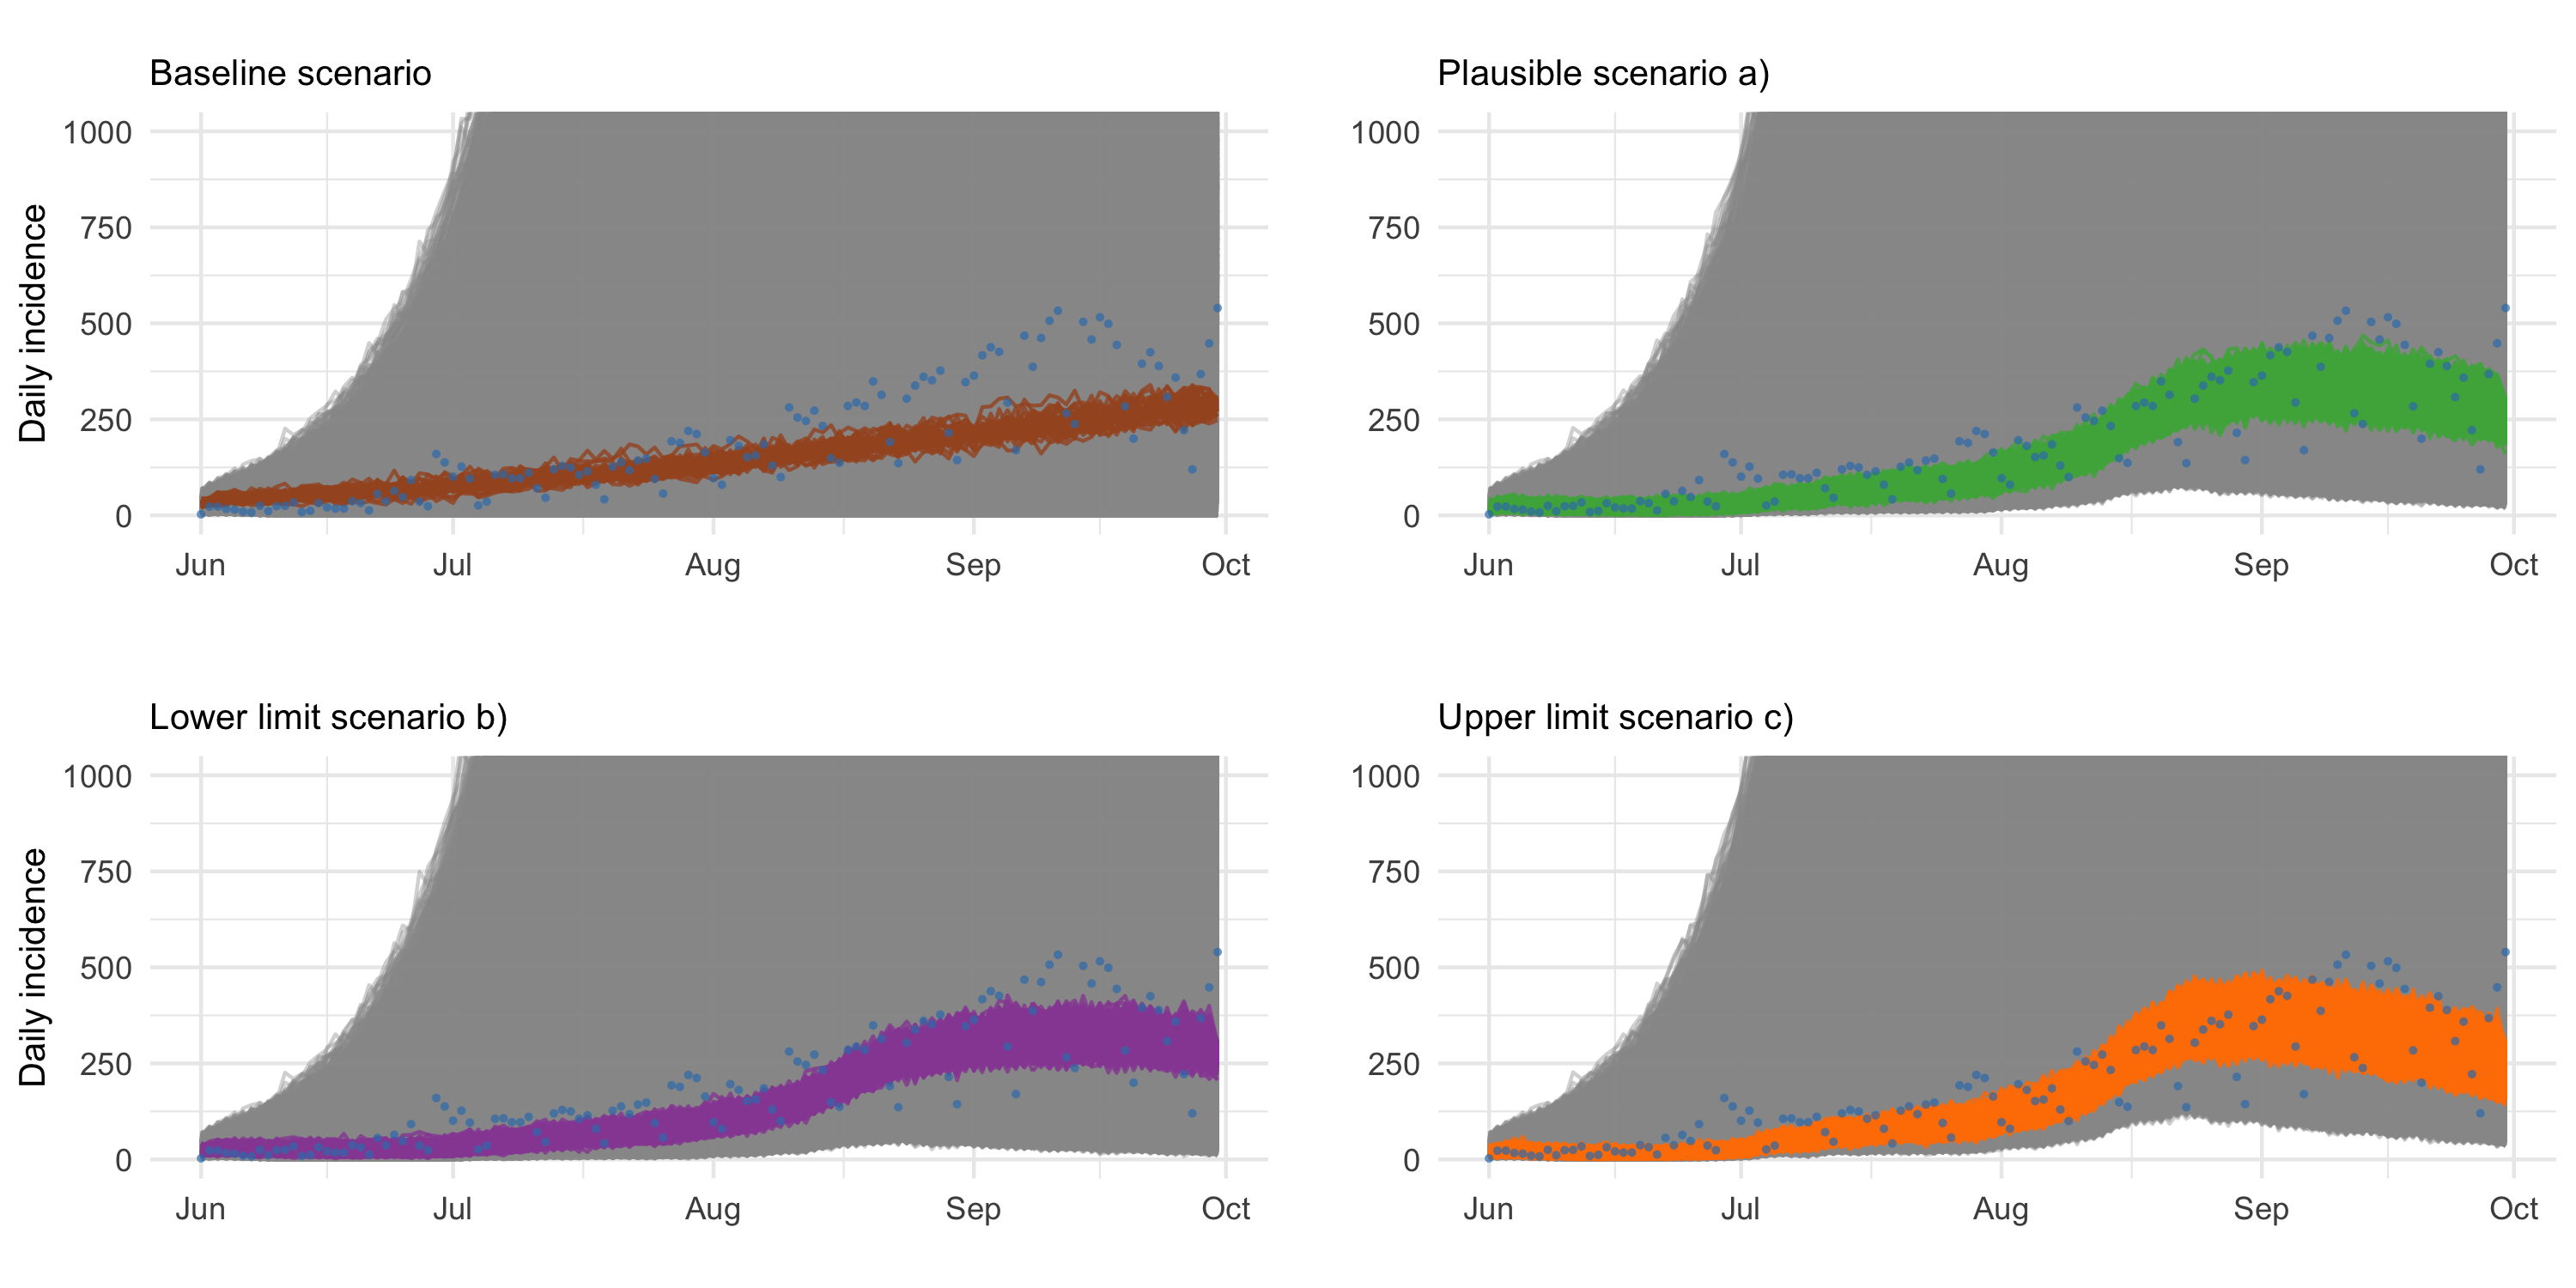
\includegraphics[scale=0.15]{Figure3_2021-06-02.png}
\caption{Accepted trajectories (coloured) using the baseline scenario (no cross-border-associated cases) and accounting for cross-border-associated cases within scenarios a-c. Blue dots show confirmed SARS-CoV-2 cases.}
\label{f3}
\end{figure*}

\section{Discussion}
The SARS-CoV-2 epidemic in Switzerland grew from a few dozen confirmed cases per day in early June 2020 to several hundred by the end of September 2020.
Ignoring cross-border-associated cases the constant $\mathcal{R}_e$ was above one for the time of interest.
In summer 2020, however, around a quarter of confirmed cases were cross-border-associated cases.
With our stochastic branching process model that accounted for cross-border-associated cases we showed that the Swiss epidemic had a $\mathcal{R}_e$ below one, i.e. a value below the critical threshold.
Also stabilisation of confirmed cases in September 2020 was captured by scenarios that accounted cross-border-associated cases if $\mathcal{R}_e$ below one.
Thus, cross-border-associated cases and their local spread was one of the leading forces that led to a 100-fold increase of confirmed cases per day within three months despite $\mathcal{R}_e$ below one.
Consequently, the impact of cross-border-associated cases cannot be ignored to understand and regulate local epidemics (during a pandemic).
\break
\par
Our stochastic branching process model was calibrated to assess the impact of cross-border-associated cases on an epidemiological, i.e. population-based, level.
For simplicity models described only Swiss epidemic and ignored geographical differences, i.e. cantons.
%We found hardly evidence that residency was associated with cross-border-associated cases (Supplementary Figure \ref{sf3}).
Stochastic effects were showed to play an important role in determining parameters in epidemics.\cite{althaus_ebola_2015,riou_pattern_2020}
Nevertheless, our method has several limitations that need to be addressed.
We did not account for variations in growth rates, seasonal effect of the SARS-CoV-2 and contact patterns, different restrictions carried out, or different incidences in groups or countries.

Our approach assumed a constant growth rate and $\mathcal{R}_e$ over the summer and ignored immunity, which was acceptable during low prevalence.
The SFOPH reported 30,883 cases before 1 June and 23,199 more until 30 September 2020.
Growth rates, can be calculated for different intervals, e.g., weeks, months, or adjusted for different factors.
For our study, a constant growth rate and $\mathcal{R}_e$ was more compatible to calculate the overall impact of cross-border-associated cases.

Our study period covered summer months only and the stringency of policy measures was constant after relaxations in June 2020.
Thus, seasonality had no influence.
However, people were more active during summer than during winter and probably more optimistic about the pandemic (mostly at the end of summer 2020), which most likely resulted in more physical contacts than before.
Tracking contact patterns, i.e., behaviour, can give a fast and good assessment of real physical distancing measures.\cite{jarvis_quantifying_2020}
Unfortunately, contact patterns were missing for this period in Switzerland.
By analysing surveillance data, we found that different age groups were exposed to the SARS-CoV-2 in different countries abroad.
Further information on age-related mixing patterns like established by the Co-Mix study is needed to better understand the social dynamics.\cite{coletti_comix_2020}
This highlights the importance of implementing and following up studies like Co-Mix.
Our study indicates that age-related mixing patterns are important to understand SARS-CoV-2 transmission.
However, close contact alone is not responsible for SARS-CoV-2 transmission.
Some transmission cluster were linked to crowded indoor spaces which underlines the possibility of aerosol (and droplet) transmission.\cite{tang_aerosol_2020}

During the time of our study, testing was free and mandatory for symptomatic cases, but not for asymptomatic cases.
If, however, a person had contact with a positive person they were required to do quarantine regardless of test results.
The contact tracing was provided either by infectees themselves, through authorities or the Swiss Covid app (launched on 15 June 2020).\cite{salath_early_2020}
Testing was not mandatory for individuals that crossed borders.
In addition, the quarantine rules in Switzerland differed by time and on the exposed country.
If people that crossed borders had to do quarantine, the level of obedience is uncertain.
Thus, hardly all cross-border-associated cases were confirmed and stopped before further transmission.
We therefore assumed that cross-border-associated cases are just as likely to transmit as local cases.
More sophisticate models adding different probabilities of further transmission inferred by in incidence of different groups, i.e., stratified by behaviour or age, might help to better understand transmission dynamics.
To be noted, if cross-border-associated cases were more likely to transmit than local cases due to a higher incidence among travellers, this would be similar to our upper limit scenario.
\break
\par
Studies reported about a two-fold and more underreporting of SARS-CoV-2 cases.\cite{Li_substantial_2020,Wu_substantial_2020}
For Switzerland, a phylogenetic analysis showed that the degree of under-ascertainment was low during summer 2020.\cite{nadeau_quantifying_2020}
Thus, the Swiss epidemic was represented well by surveillance data.
%Nevertheless, the increase of cases could still be changed due to reporting changes.
%By ignored the delay of confirming cases, our simulations reflected the day of testing and not the start of infection.

From our findings travel strategies might be derived, including mandatory quarantine and test strategies for the coming summer 2021.
Also in other countries, travel and resulting new introduction had a strong impact on the local epidemic.\cite{worobey_emergence_2020,russell_effect_2021,hodcroft_emergence_2020}
Most likely (global) herd immunity will not be achieved in the summer 2021, so existing measures such as testing and physical distancing remain important to keep incidence low.
In addition, there is still uncertainty about asymptomatic cases.\cite{nogrady_what_2020,buitrago-garcia_occurrence_2020}
Studies found the proportion of asymptomatic cases to be 17\% (or 20\%) and 1/4 less transmissible.\cite{byambasuren_estimating_2020,buitrago-garcia_occurrence_2020,bi_household_2020}
It could be an option to test all that cross borders and give them the option of reduced quarantine for negative cases.\cite{ashcroft_quantifying_2021}
Mandatory quarantine and testing might reduce the willingness to travel as it includes extra expenses for travellers and keeps awareness of the SARS-CoV-2 pandemic high.
Travel mobility might be reduced, and cross-border-associated cases and their local spreading might be minimised through testing and mandatory quarantine.
Here we need to emphasised that one case might lead to an outbreak thus population based surveillance including reporting of countries of exposure and viral sequence data is crucial for appropriate measures.\cite{worobey_emergence_2020}
Worbey et al., highlighted the need to detect new introduction and transmission clusters early through routine, massive, sequence based approaches — not months or years later, when clinical symptoms have accumulated.\cite{worobey_emergence_2020}
For Switzerland in summer 2020 incidence was low compared to other countries.
Thus, with small and light travel measures, a large number of cases were introduced to the local epidemic.
Finally, Switzerland paid a high price due to light measures that eventually induced a growing epidemic through cross-border-associated cases.
\break
\par
Switzerland is a relatively small country with few million citizens, but due to its location (and its wealth) there is a high potential for travel which had impact on the Swiss epidemic.
Quantifying the role of cross-border-associated cases on the national dynamics of SARS-CoV-2 epidemics is important to understand transmission.
%In Switzerland, cross-border-associated cases have had a considerable impact on the national dynamics and could explain the growth of the SARS-CoV-2 epidemic during summer 2020.
Our results underline the importance of improved surveillance for (international) travellers in order to better control the spread of SARS-CoV-2.


\section{Acknowledgement}
We thank the Swiss FOPH (http://www.bag.admin.ch) and the UBELIX team. Calculations were performed on UBELIX (http://www.id.unibe.ch/hpc), the HPC cluster at the University of Bern.

\section{Author contributions}
MLR, EBH, JR, NAR, and CLR conceived the study and contributed to the analysis of the results.
MLR performed the analysis and wrote the first draft of the manuscript.
NH gave important inputs for the analysis and interpretation.
All authors read and approved the final manuscript.

\section{Funding}
European Union’s Horizon 2020 research and innovation programme - project EpiPose (No 101003688). Swiss National Science Foundation (grant 196046).

\section{Reference}
\bibliography{../manuscript/su2020_cov2.bib}
\bibliographystyle{vancouver}

\end{multicols}

\clearpage
\begin{suppfigure}[h]
\centering
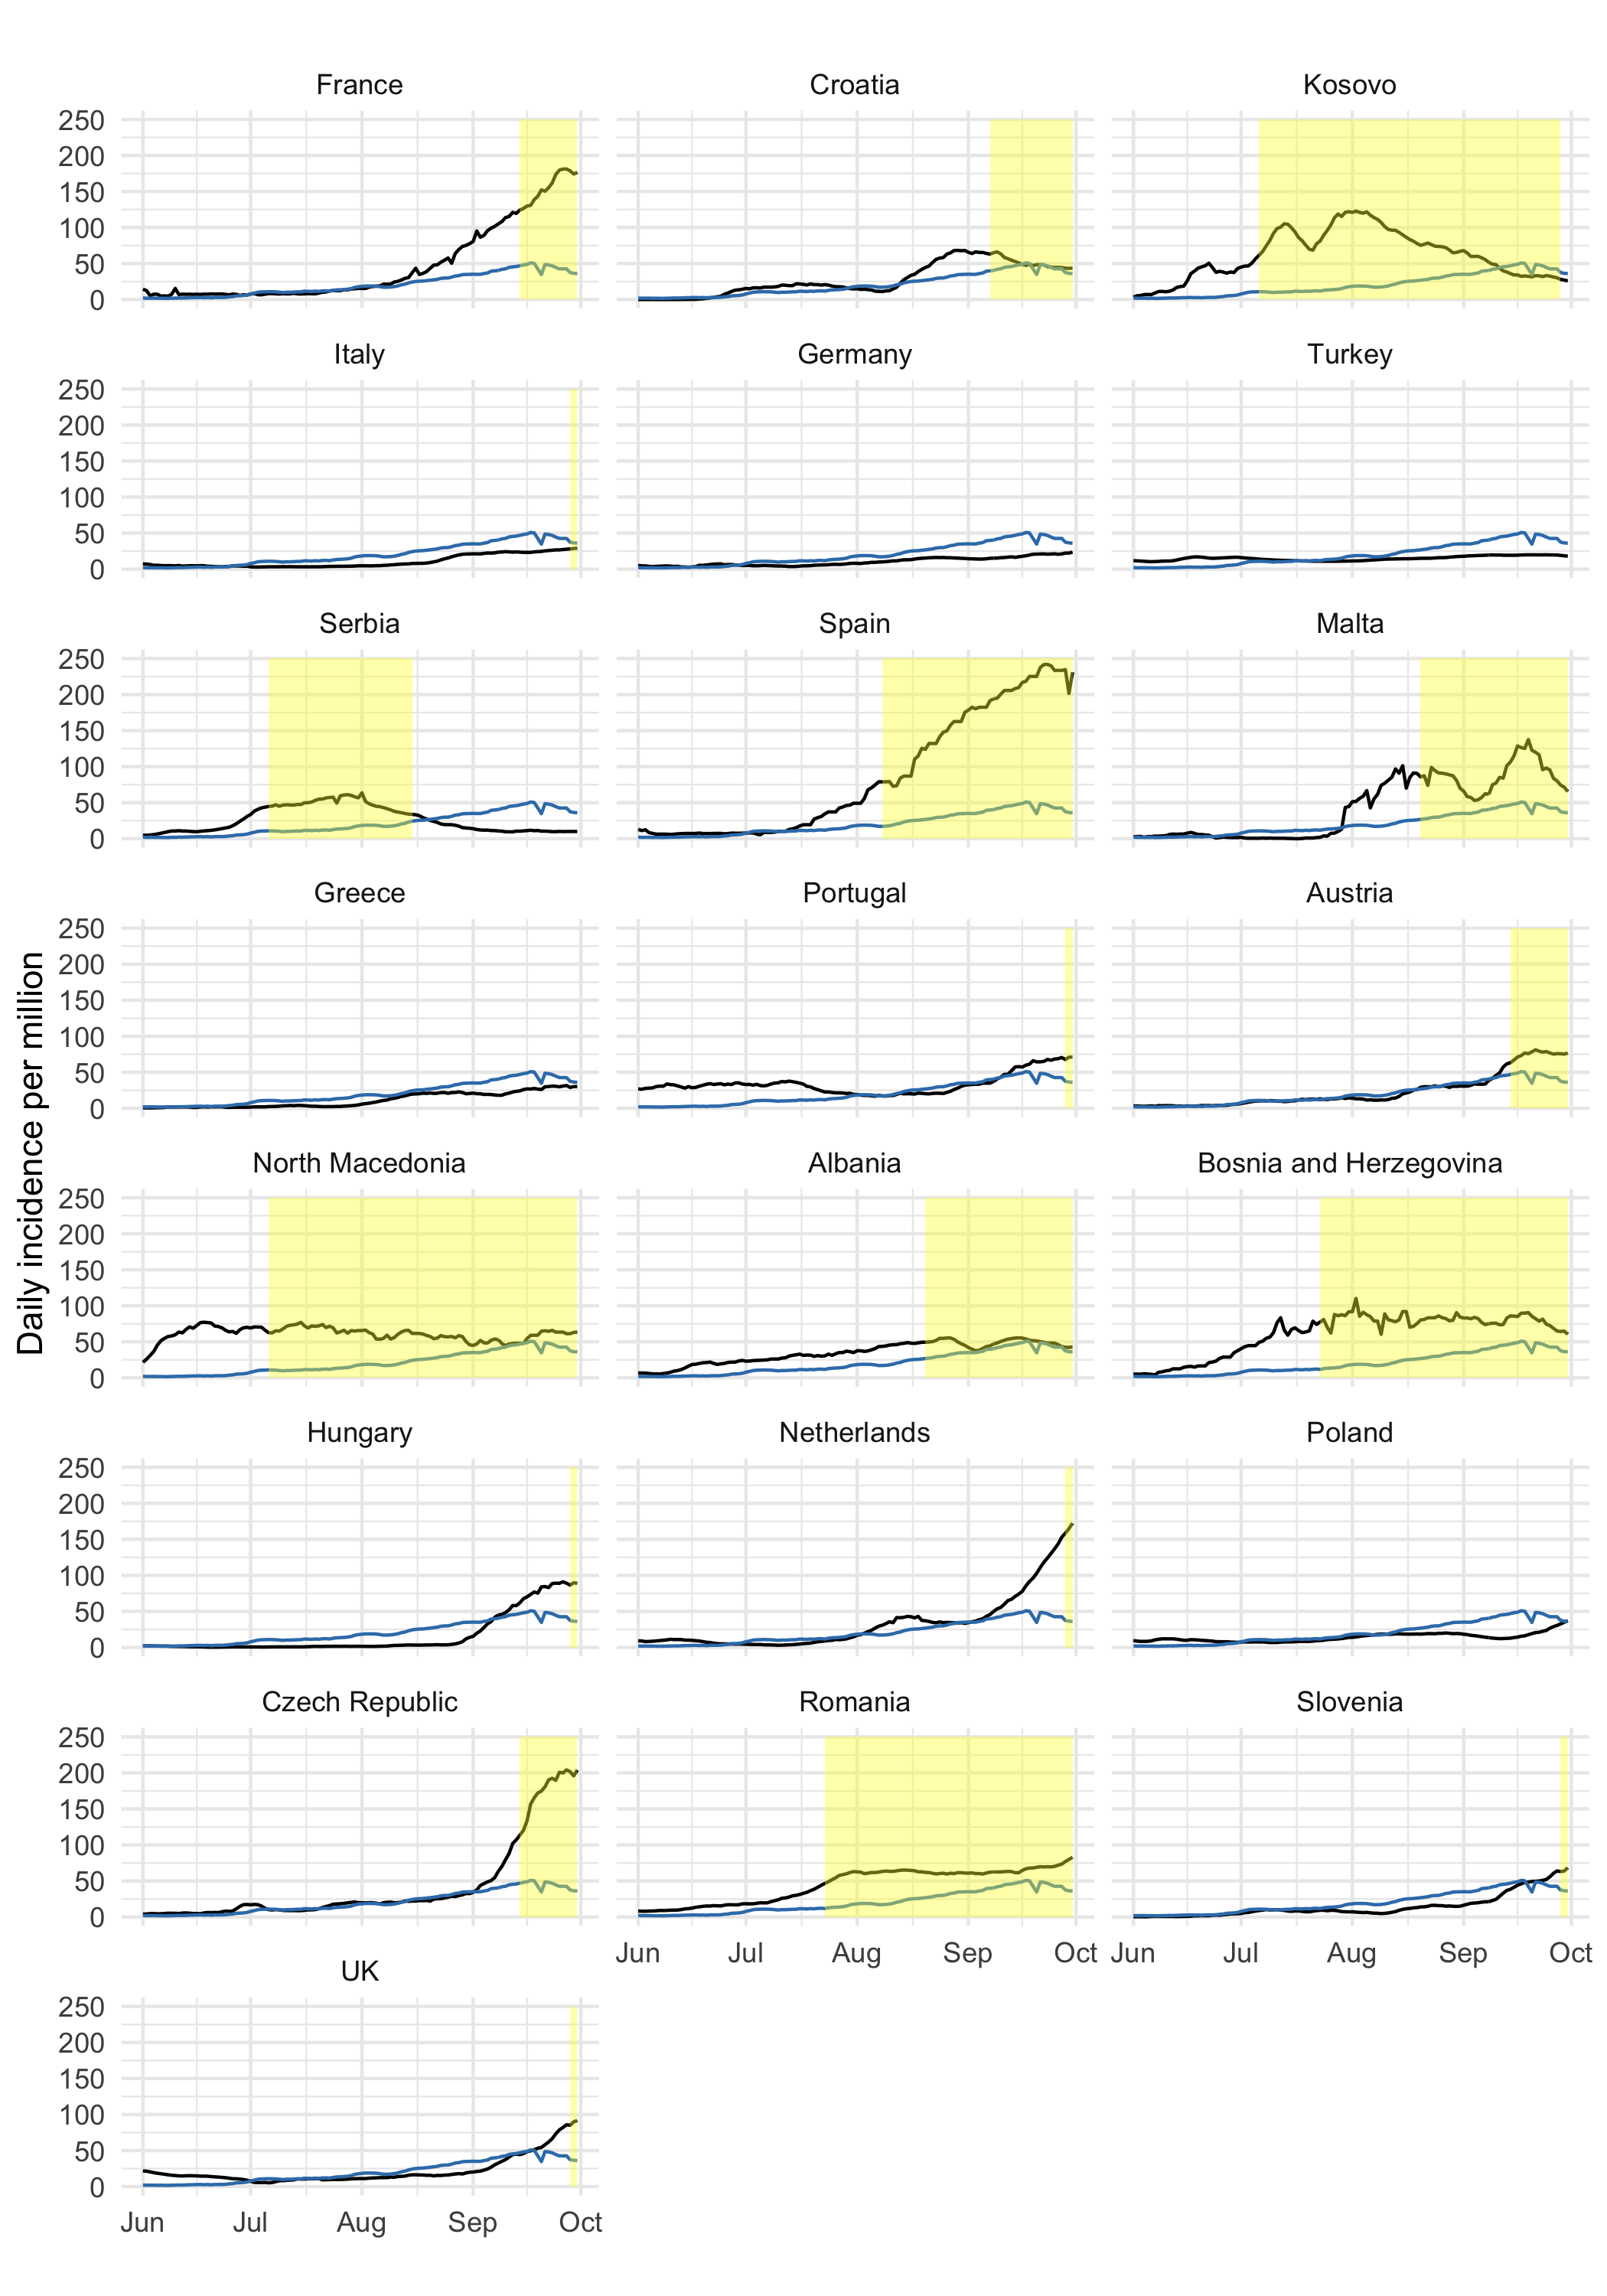
\includegraphics[scale=0.125]{SF1_2021-06-02.png}
\caption{Daily incidence per million compared to Switzerland (in blue). Yellow area represent when country was on the mandatory quarantine list whereby their was regional differences for France, Austria, and Spain.}
\label{sf1}
\end{suppfigure}

\clearpage
\begin{suppfigure}[h]
\centering
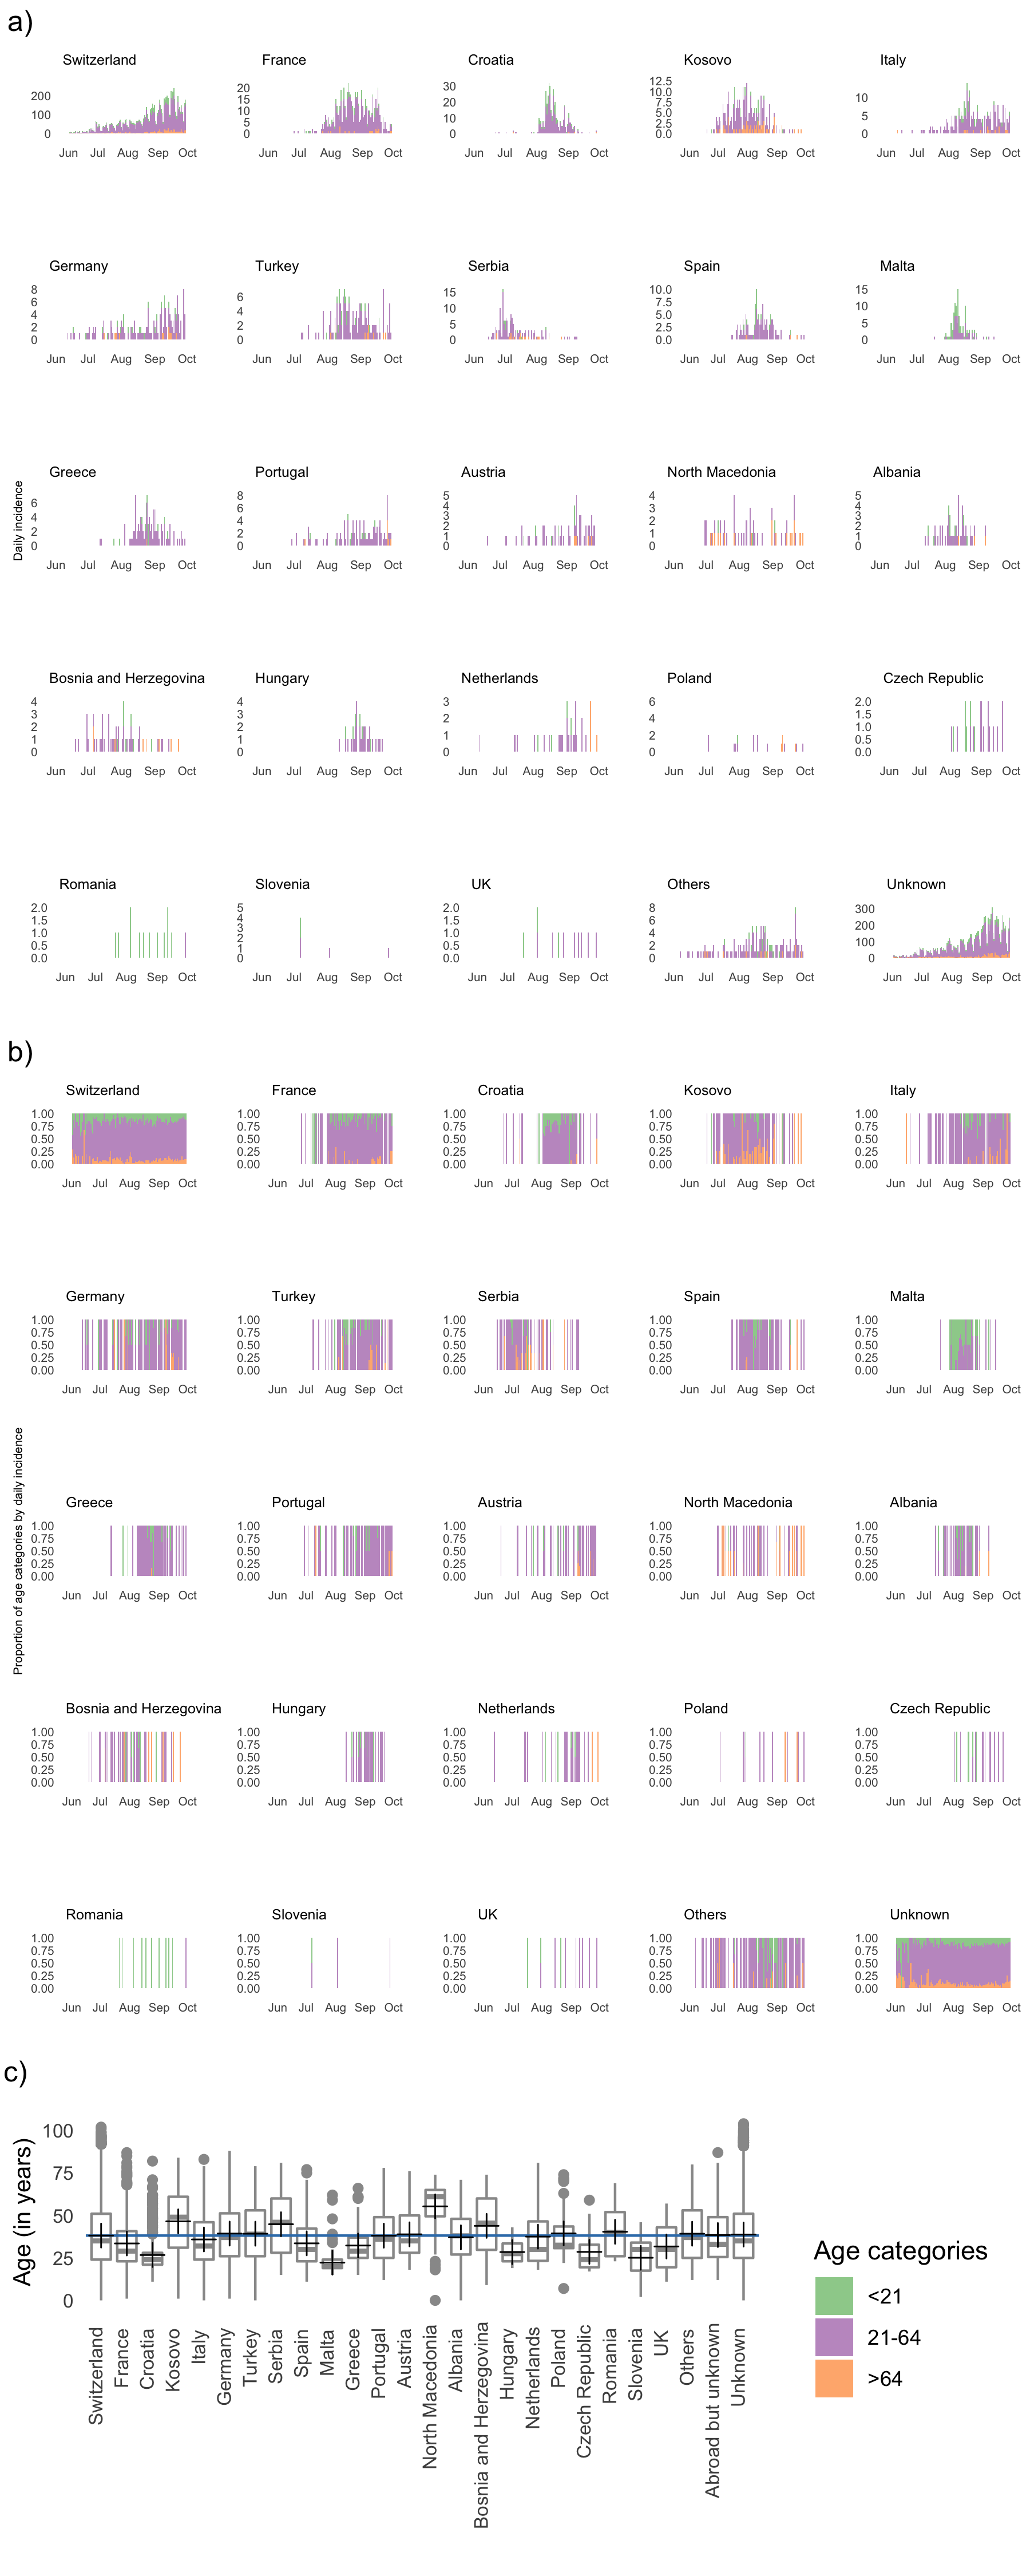
\includegraphics[scale=0.125]{SF2_2021-06-02.png}
\caption{Reported cases and the most likely country of exposure.
a) Reported cases and fraction of different age groups.
b) Proportion of all cases and fraction of different age groups.
c) Age distribution for reported cases according to their reported most likely country of exposure (ordered by number of cases).
+ represents the mean age; horizontal line is the mean age of individuals that were only exposed in Switzerland.}
\label{sf2}
\end{suppfigure}


\clearpage
\begin{suppfigure}[h]
\centering
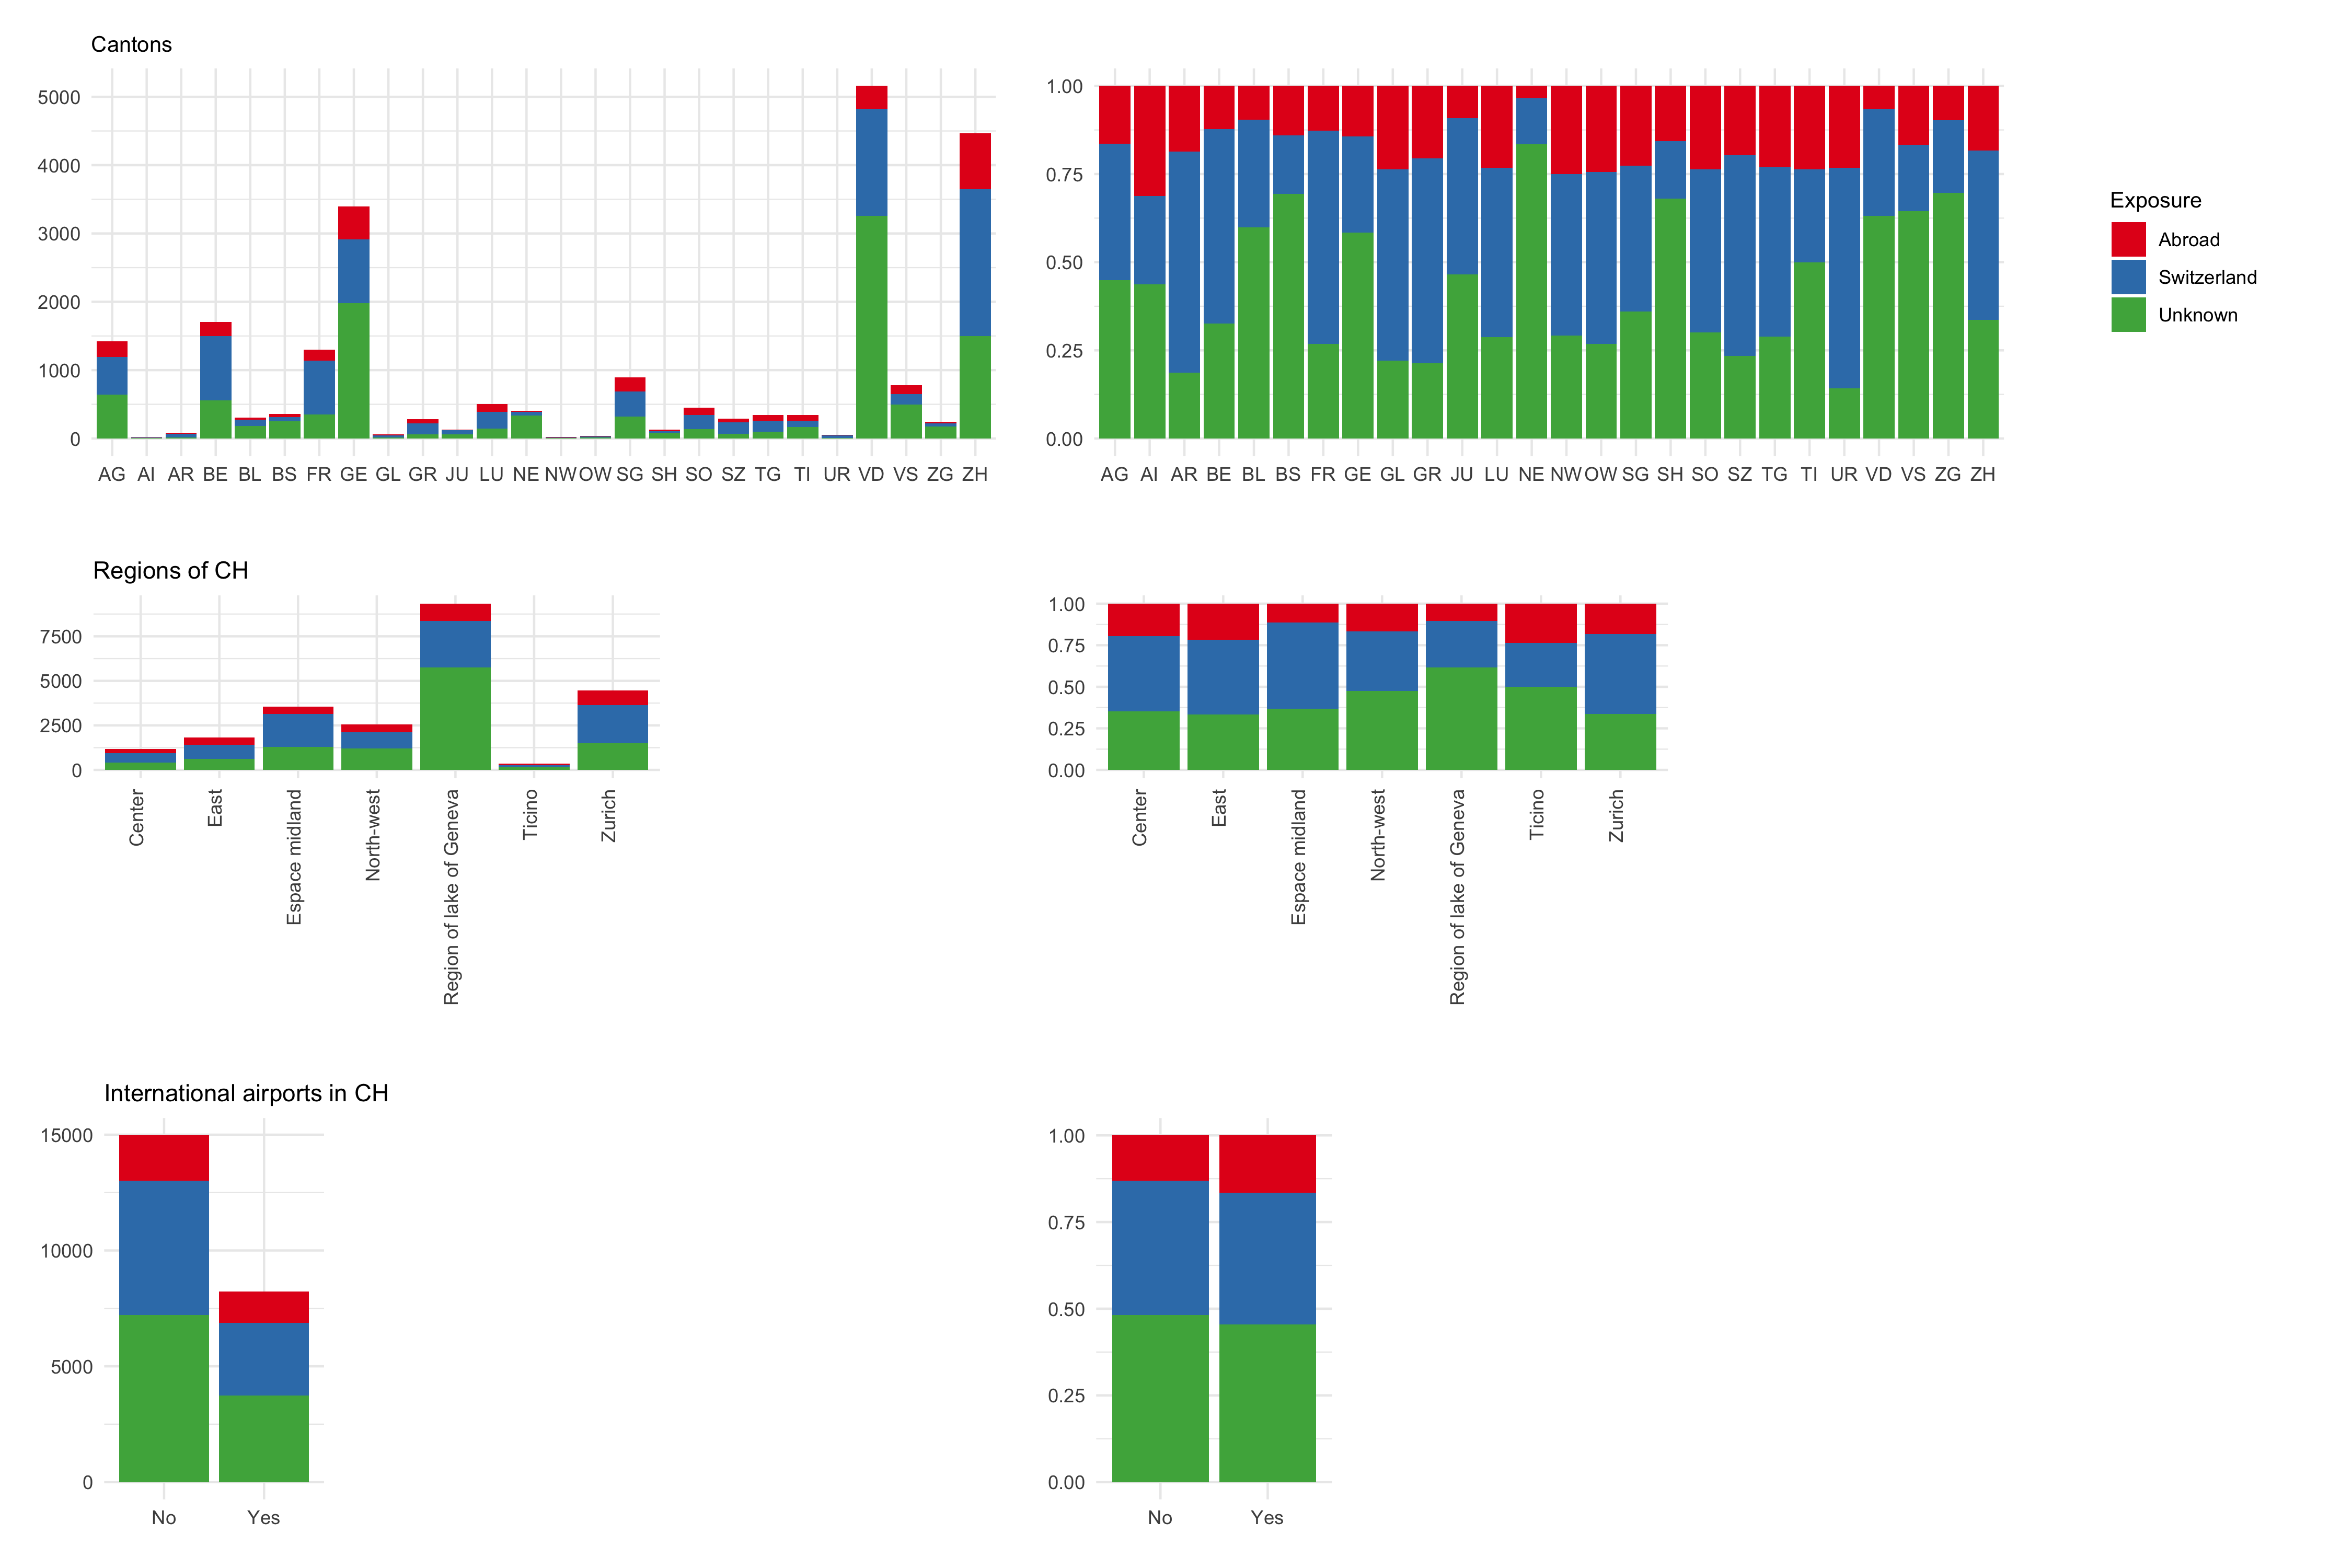
\includegraphics[scale=0.1]{SF3_2021-06-02.png}
\caption{Country of exposure and region of cases' residency.}
\label{sf3}
\end{suppfigure}


\end{document}
